\chapter[\'Etude clinique]{\'Etude clinique}

%Souvenons-nous brièvement de l'évolution de la signification du terme
%``clinique'' enraciné dès l'Antiquité.
%A l’origine,\textbf{ l’activité clinique} (<gr. klinê = le lit) est celle du médecin qui, au chevet du malade, procède à l’examen des manifestations de la maladie (méthode de l’observation, de l’interrogation et de l’écoute) en vue de poser un diagnostic*, un pronostic* et une prescription* de traitement.
%Michel Foucault (1926-†1984), psychologue français, dans son ouvrage capital de 1963,
%«Naissance de la clinique» nous rend attentifs au fait que l’adjectif «clinique» fut longtemps du monopole médical, avec %l’observation « naturelle » faite au lit du malade, uniquement à l’aide des organes sensoriels.

%Hippocrate (médecin grec, Cos 460-377) était clinicien : il apprenait à ses étudiants l’art d’observer les symptômes, ceux-ci étant les réactions d’une personnalité à une agression pathogène. Généralisation et rationalisation, selon les critères d’Aristote, permettaient l’élaboration de « ces entités nosologiques* », les maladies, qui s’emparaient du corps du malade et poussant les médecins, exorcistes laïques, à les en faire sortir.
%Les publications de Th.Ribot à la Sorbonne rejoignent [avec «La psychologie des sentiments »(1896), «Les maladies de la mémoire »(1883) et «Les maladies de la personnalité » (1885)], les idées de S. Freud, montrant la primauté de la vie affective, où les tendances inconscientes jouent un rôle fondamental, et pouvant s’extérioriser soit par l’arrêt du développement affectif, soit par la dissolution des acquisitions plus récentes.

%L’expression « psychologie clinique » apparaît sous la plume de S. Freud, dans sa lettre à W. Fliess du 30.01.1899 : « Maintenant, la connexion avec la psychologie, telle qu’elle se présente sur les Etudes sur l’hystérie(1895) sort du chaos, j’aperçois les relations avec le conflit, la vie, tout ce que j’aimerais appeler psychologie clinique ». 

%La définition « officielle » de la psychologie clinique mobilise et articule la singularité et
%la totalité, de façon à reconnaître une discipline psychologique basée sur l’étude approfondie des cas individuels, l’étude de la conduite humaine individuelle et de ses conditions (hérédité, maturation, conditions psychologiques et pathologiques, histoire de la vie), en somme, l’étude de la personne totale «en situation», c.à.d. l’expérience vécue de ce rapport à l’environnement.

%Au vue de cet aperçu historique, on peut reconnaître que
%dans certains milieux psychiatriques actuels, la musicothérapie trouve plus sa place aussi dans le complètement des tableaux cliniques.

Dans notre étude, l'axe principal porte sur la
vérification de l'amélioration de
la capacité d'écoute suite au travail musicothérapeutique.
Nous allons
d'abord exposer le cadre dans lequel nous avons fait ces tests, la
population étudiée et procéder à la comparaison des modifications de
l'écoute.

\section{Méthode}

 La clinique privée (Privatklinik)
de Meiringen (BE) est  principalement spécialisée en
addictologie avec problèmes d'alcool et de toxicodépendance, couvrant aussi les aspects dépressifs
et les
burnouts.


Elle dispose d'une capacité de 195 lits, et le temps de séjour fluctue de 3 à 6 semaines ou plus, en
fonction de la participation des assurances.

Actuellement, en plus de l'administration et l'intendance, les 33
médecins et psychiatres, sont
accompagnés par 177
soignants, dont infirmiers psychiatriques, aide-infirmières, physio et
ergothérapeutes, 
psychologues et intervenants en \textit{thérapies
créatives}, comme l'art-thérapie, thérapie
corporelle, zoothérapie (chien/cheval),  ateliers de créativité --
bois et terre --,  les textiles et la\textbf{ musicothérapie} avec deux
personnes, dont la souscrite à titre de 10 pour cent.


%\textbf{Organigramme}: nous avons obtenu l'autorisation de vous
%montrer l'organigramme de la Clinique de Meiringen lors de la
%soutenance.




%(-OH*:  le radical hydroxile, oxydrile de la molécule éthylique)


\subsection{Population}
L'\textbf{échantillonnage} fortement conditionné par les contraintes
institutionnelles, comme les interruptions prématurées de séjour, les rendez-vous
 médicaux superposés, l'impossibilité de participation physique et/ou
 psychique, les remplacements disparates et hétéroclites de ma
 collègue, l'emploi à
 temps partiel, a été restreint  par le choix d'un nombre limité de
 patients (N=29).
Une autre contrainte de nature extra-institutionnelle allant dans le
même sens réside dans l'éloignement géographique.

\textbf{Le Groupe Musicothérapeutique (expérimental) GM} comporte 21
patients, dont 6
femmes et 15 hommes.

\textbf{Le  Groupe Contrôle GC} comporte 8 patients, dont 4 femmes et 4 hommes.

Le nombre
des patients s'est limité  à 8
patients (4 hommes/4 femmes) pour le GM, et à 7 patients (4 hommes/3
femmes) pour le GC pour obtenir une comparaison entre les tests et les questionnaires.




En synthèse:
 \begin{itemize}
 
 \item \textbf{Nombre total de personnes}: N= 29 
\item\textbf{Genre et âge de la population étudiée:}  19 hommes et 10 femmes, de 25 à 72
  ans dont l'âge moyen est de 48 ans.
 \item\textbf{Pathologies}: troubles de la régulation émotionnelle
   dont le burnout, les dépendances, la dépression.
   Il n'a pas été
   possible de différencier les pathologies, car la pose de
   diagnostic dans ce domaine reste toujours difficile et délicat pour le corps médical, raisons pour lesquelles elles
   se trouvent traitées ensemble.
 \item \textbf{Total de séances} par personne en
   musicothérapie= 4 ;   \textbf{mu}=1/semaine;  
 \textbf{t}= 50--60 min, période = 3 -- 4 semaines.
\end{itemize}




 %mu en grec
\subsection{Démarches}
Obtenu l'aval de la direction de la
clinique pour cette étude,  le personnel soignant et l'ensemble des
thérapeutes (ateliers, thérapies créatives, kynési--cyno--
et hippothérapie) vont être informés aussi par écrit.

Ce même texte, destiné aux
patients\footnote{Cf.Annexe A.7} explique le projet de l'étude sur l'écoute, comme aussi la transformation
avec ou sans musicothérapie.
Le consentement libre est validé par la signature du patient, après
un court entretien avec lecture.\footnote{Cf. Annexe A.10}.
%\footnote{Regula
  %Lehmann, musicothérapeute  à 90\%  à la clinique de Meiringen.} 


Après ces prémisses, l'étude commence véritablement avec l'application du test
audiométrique suivie du questionnaire qualitatif.

\textbf{L'étude} est
réalisée en fonction des séjours variables des patients, soit une
totalité  de quatre semaines
distribuées dans l'intervalle juin --
octobre 2017,  à l'aide de tests et questionnaires appliqués en début
et fin de séjour.

\textbf{Types de thérapie, musicothérapie} réceptive et/ou active.
Les autres formes de thérapies, en gardant
leur indépendance par rapport à notre analyse, se déroulent simultanément, à
l'exception de la musicothérapie pour le groupe contrôle.


\subsection{Matériel (tests et questionnaires)}
	Nous utiliserons deux tests différents : 
	le test d'écoute spécifique d'Alfred Tomatis
	et le test-questionnaire, le WHO QOL-Bref, les deux qualitatifs et quantitatifs.

        
        \textbf{Le test d'écoute}
        \footnote{Cf. Ch. 3. A. Tomatis p.27} détecte la manière de recevoir
        l'information. 
Nous obtenons une  
	\textbf{représentation graphique} générale des courbes de l'écoute
        (équilibre, déséquilibre, harmonie) à partir des seuils d'écoute
        calculés selon les fréquences et le volume que le sujet entend
        avec des zones à lire et interpréter.
	A cet effet, nous utiliserons l'appareil conçu à partir de 1950 par Alfred Tomatis, médecin
        O. R. L.: le Hearing Test, ou TLST, testant
        l'écoute pré/post-thérapie
        afin d'établir une comparaison.
        L'utilisation particulière du \textit{test de perception d'écoute de Tomatis}  est
légitimée par sa facilité et  simplicité d'application, en dehors de
son contexte thérapeutique.\footnote{Nous précisons qu'aucun support de la méthode conçue par
        Tomatis n'interviendra pendant les séances de musicothérapie.}
      Nous pourrons constater
      s'il existe un changement dans l'écoute du sujet grâce au support graphique, tel un ``dessin'',
      une image. %fournissant des critères d'analyse.
      
        Le\textbf{ WHO QOL  - Bref:  World Health
   Organisation Quality of Life Assessement } (Cf. Annexe A.9.) est un test d'évaluation de la qualité de vie, issu du
	programme de l'Organisation Mondiale de la Santé, l'OMS.
	Ce questionnaire est réalisé en parallèle, rempli par
        les patients eux-même à l'entrée de leur séjour en clinique et
        à leur sortie, avec ou sans musicothérapie.
 L'utilisation de ce questionnaire a pour but d'avoir
 une variable supplémentaire pour confirmer ou infirmer en
parallèle l'action supposée  de la musicothérapie sur une éventuelle
modification de l'écoute.

Il sert aussi à constater s'il y a une\textbf{ transformation psychique }du sujet,
 (positive ou négative) et s'il existe une \textbf{corrélation }de
 résultats avec le test d'écoute.

 
        L'estimation se fait à partir d'une échelle
d'auto-évaluation subjective avec 26 questions courtes 
--il s'agit ici de la version courte  la plus récente (2004) du questionnaire
 WHOQOL-100 datant de 1998, --
dont un item concernant la qualité de vie globale
auto-évaluée par le sujet, un item évaluant la santé générale perçue
et les 24 autres se répartissent selon les 4 domaines suivants: physique, psychologique, relations sociales et environnement.
\begin{enumerate}
\item  Le domaine de la perception physique (7 items) comprend l' activité quotidienne// la dépendance et/ou l'assistance médicale// la fatigabilité, l'énergie//la mobilité// la douleur// le sommeil// la capacité de travail//
	\item Le domaine psychologique (6 items):  image de soi, apparence// ressentis positifs et négatifs// estime de soi// spiritualité, croyances personnelles, religion// mémoire et concentration, apprentissage, pensée.
		\item Le domaine des relations sociales (3 items) : relations personnelles// soutien social// vie sexuelle.
			\item Le domaine de l'environnement (8 items) :
                         l'environnement domestique et physique
                         (pollution, bruit, trafic, climat)// la
                         situation financière//  la liberté, la
                         sécurité physique et morale//
                         l'accessibilité et qualité de la santé// les
                         opportunités de détente, loisirs, accès aux
                         informations// logement et transport// 
\end{enumerate}
		Les questions varient selon sa propre perception, telle la satisfaction
au sujet de son  sommeil, de sa vie relationelle, sexuelle, de
l'opinion que l'on a sur soi, \textit{`` Êtes-vous satisfait de
vous-même?'' , ``Acceptez-vous votre apparence physique?''} par
exemple, ou si le patient éprouve souvent des sentiments négatifs
et s'il a assez d'énergie dans la vie de tous les jours.
La cotation se fait sur 4 types d'échelles de réponses en 5 points (de 1 à 5)
permettant l'évaluation de l'intensité, la fréquence, la capacité, l'évaluation.
Le patient le remplit avec ou sans aide du
thérapeute lors de chaque test
d'écoute.

La figure suivante décrit de manière succinte le déroulement de
l'étude sur la durée avec les deux groupes.



        \begin{figure}[hb]
\centering
\includegraphics[width=0.7\linewidth]{images/Groupecontrole.png}
\caption[Schéma du déroulement]{Déroulement de l'étude avec GM et GC}
       
%\label{groupecontroleimage1}
\end{figure}
	
 \subsection{Procédure}
Chaque participant du groupe GM et GC va faire en entrée et en sortie de
clinique, après environ 4 semaines, un
          test avec questionnaire  WHOQOL. (GC ayant suivi une musicothérapie active et/ou réceptive (1x par
        semaine).\footnote{Voir Fig. 4.1.}
          Chaque test d'écoute dure
        70 à 90 minutes, fait 2x (pré/post-thérapie) et 
        suivi du questionnaire WHOQOL (2x10') rempli par le
        patient lui-même.
        
Sur \textbf{44 tests d'écoute} réalisés pour \textbf{GC et GM},
      nous avons décompté\textbf{ 30 tests} valides qui serviront de
     comparatif dont \textbf{16} pour
     GM, groupe de musicothérapie et \textbf{14 tests d'écoute} pour GC, le groupe
     contrôle.
      \begin{figure}
\centering
\includegraphics[width=1\linewidth]{images/graphiques/test_ecoute.jpg}
\caption[Schéma du déroulement]{Nombre de tests d'écoute avec GM et GC}
       
%\label{groupecontroleimage1}
\end{figure}

Sur \textbf{25 questionnaires WHOQOL}, il y a \textbf{10 pour GM} remplis
avec 8 pré- et seulement 2
     post- thérapies; et \textbf{15 pour GC} dont 8 pré-
     et 7 post-thérapie.
      Nous avons dans l'ensemble un total de \textbf{9 questionnaires} pour le
     comparatif des 2 groupes réunis.
    
\textbf{ Pathologie des groupes}: Les patients ont été répartis en deux groupes sans différenciation de
 leur pathologie. Nous avons conscience d'avoir mélangé des symptomatologies qui
 toutefois paraissent
 sous-tendues par
                                               certains mécanismes
                                               similaires dont le
                                               noyau commun est une
                                              \textbf{difficulté de
                                               régulation des
                                               émotions}, 
                                               s'exprimant par une
                                               humeur négative.
                                               Il convient ici de mentionner que, en vue de la taille réduite des échantillons, il n'est pas
pertinent de se lancer dans une analyse purement
quantitative.

\section{Hypothèses opérationnelles}

Il s'agit ainsi d'une étude mixant le \textbf{quantitatif  et le
  qualitatif}.
En procédant toujours en amont et en aval, --pré/postpostthérapie--, nous
avons obtenu la \textbf{moyenne} \textbf{des seuils
auditifs de la c.a. et de la c.o.} de l'oreille \textbf{droite} et de
l'oreille \textbf{gauche} de chaque patient, ci-dessous illustrée par
plusieurs exemples. Ensuite, après avoir 
fait une comparaison des dessins des différentes courbes et
décompté le nombre des croisements, l'ensemble des résultats sera analysé et comparé.
Nous ferons ensuite la corrélation des résultats avec ceux du\textbf{
  WHOQOL}.

Qu'il s'agisse des tests ou des questionnaires, nous avons choisi de
simplifier les \textbf{résultats} sous forme de signes
mathématiques, $+$, $=$, $-$ avec les significations suivantes.
Avec les \textbf{tests d'écoute}: 
\begin{enumerate}
\item$+$   : amélioration, modification;  rapprochement significatif à la courbe dite idéale.
\item$=$   : amélioration insignifiante, correspond à : $+/-$, (si c.a. $ + $ et c.o. $-$, ou vice-versa).

\item$-$   : pas d'amélioration et pas/trop peu  de modification, inversion
des courbes (c.o. supérieure à c.a.). 

  Avec les \textbf{croisements}, les chiffres des 2 tests pré/post
  nous permettent d'obtenir une comparaison: 
  \item Plus petit est le nombre, meilleur est le résultat, ce qui correspond à un signe positif : $+$.
\item Dans le
  cas contraire, ce sera un signe négatif: $-$.
  
\end{enumerate}


 \subsection{ Comparaison pré/post-thérapie des résultats du test d'écoute}
Avec les tests d'écoute, nous 
allons donc prendre en compte:

\begin{enumerate}
 \item   les \textbf{seuils} auditifs --moyenne
représentée sous forme des \textbf{courbes aérienne et osseuse} --
\item  l'observation par \textbf{comparaison graphique des différentes
  courbes}
\item le nombre de
\textbf{croisements}.\footnote{Cf. Ch. 3 A. Tomatis p. 26: les distorsions}
 
\end{enumerate}


%\textbf{Index courbe idéale aérienne et osseuse}:
%La moyenne chiffrée de la courbe aérienne: 1,3
%La moyenne chiffrée de la courbe osseuse: 3,11


  Nous allons commencer par l'observation de trois patients du Groupe Contrôle.
     

      \textbf{Groupe Contrôle : Observation avec 3 patients}
  \paragraph{ A. Patient Br.:}
  \begin{figure}[ht]
\centering
\includegraphics[width=0.7\linewidth]{images/graphiques/bru_pre.png}
\caption[Moyenne OG+OD]{Premier test Br.}
       
%\label{groupecontroleimage1}
\end{figure}



 \begin{figure}[th]
\centering
\includegraphics[width=0.7\linewidth]{images/graphiques/bru_post.png}
\caption[Moyenne OG+OD]{Second test Br.}
       
%\label{groupecontroleimage1}
\end{figure}

	\begin{enumerate}
 		\item  c.a.: pas de modification, augmentation des
                  seuils: $-$
 		\item  c.o.: redressement des seuils: $+$
 		\item  croisements: $5/4$ : $+$ : ce qui signifie:  5 croisements lors du 1°test// 4 croisements lors du 2° test= nous avons 1 croisement en moins, donc le résultat est considéré comme positif en fin
                  de séjour.
                \end{enumerate}

                \textbf{  Conclusion:  -    +    +       :  +}




\paragraph{B. Patient Sch.:}

	\begin{enumerate}
 		
 		\item : c.a.: pas de modification, très légère augmentation des
                  seuils: +/-
 		\item : c.o.: a passé sous c.a., modification des seuils: +
 		\item : croisements: 2/2 :     =
                   \end{enumerate}
 \textbf{  Conclusion:  +/-    +    =        :  =}

\begin{figure}
\centering
\includegraphics[width=0.7\linewidth]{images/graphiques/schaff_pre.png}
\caption[Moyenne OG+OD]{Premier test Sch.}
       
%\label{groupecontroleimage1}
\end{figure}


         \begin{figure}
\centering
\includegraphics[width=0.7\linewidth]{images/graphiques/schaff_post.png}
\caption[Moyenne OG+OD]{Second test Sch.}
       
\label{groupecontroleimage1}
\end{figure}


\paragraph{C. Patient Wal.:}



\begin{figure}
\centering
\includegraphics[width=0.7\linewidth]{images/graphiques/wal_pre.png}
\caption[Moyenne OG+OD]{Premier test Wal.}
       
%\label{groupecontroleimage1}
\end{figure}

	\begin{enumerate}
 		
 		\item : c.a.: peu de modification: =
                
 		\item : c.o.: reste dominante, tentative de rapprochement de c.a.: -
 		\item : croisements: 1/3 :  -
                  
                \end{enumerate}

                \textbf{ Conclusion:  $= -  -        : -$ }

               \begin{figure}
\centering
\includegraphics[width=0.7\linewidth]{images/graphiques/wal_post.png}
\caption[Moyenne OG+OD]{Second test Wal.}
       
\label{groupecontroleimage1}
\end{figure}
                
  \textbf{ Groupe de Musicothérapie: Observation avec 4 patients}

\paragraph{ A. Patient Sw.:}



 \begin{figure}[th]
\centering
\includegraphics[width=0.7\linewidth]{images/graphiques/sw_pre.png}
\caption[Moyenne OG+OD]{Premier test Sw.}
       
%\label{groupecontroleimage1}
\end{figure}

	\begin{enumerate}
 		
 		\item : c.a.: pas de modification: = %  1,27/1,27
                
 		\item : c.o.: redressement et rapprochement,
                  relèvement des seuils: -       %  3,07/3,39
 		\item : croisements: 1/3 :  -
                  
                \end{enumerate}

                \textbf{  Conclusion:  = +  -        : ``=''}

                \begin{figure}
\centering
\includegraphics[width=0.7\linewidth]{images/graphiques/sw_post.png}
\caption[Moyenne OG+OD]{Second test Sw.}
       
%\label{groupecontroleimage1}
\end{figure}




\paragraph{B. Patient Cav.: }

(pas de WOQOL fin de séjour)


\begin{figure}[th]
\centering
\includegraphics[width=0.7\linewidth]{images/graphiques/cav_pre.png}
\caption[Moyenne OG+OD]{Premier test Cav.}
       
%\label{groupecontroleimage1}
\end{figure}

	\begin{enumerate}
 		
 		\item : c.a.: redressement: +
                
 		\item : c.o.: redressement et rapprochement, relèvement des seuils: +
 		\item : croisements: 3/1 :  +
                  
                \end{enumerate}

                \textbf{  Conclusion:  + + +       : ``+''}

                \begin{figure}
\centering
\includegraphics[width=0.7\linewidth]{images/graphiques/cav_post.png}
\caption[Moyenne OG+OD]{Second test Cav.}
       
%\label{groupecontroleimage1}
                \end{figure}



                
               \paragraph{ C. Patient M.:}


	\begin{enumerate}
 		
 		\item : c.a.: redressement: : +   % 6,43/6,03
                
 		\item : c.o.: redressement et rapprochement,
                  relèvement des seuils:  +     %6,25/5,85:
 		\item : croisements: 3/3 :  =
                  
                \end{enumerate}

                \textbf{  Conclusion:  +  +  =     : ``+''}

                \begin{figure}
\centering
\includegraphics[width=0.7\linewidth]{images/graphiques/m_pre.png}
\caption[Moyenne OG+OD]{Premier test M.}
       
%\label{groupecontroleimage1}
\end{figure}


                        \begin{figure}
\centering
\includegraphics[width=0.7\linewidth]{images/graphiques/m_post.png}
\caption[Moyenne OG+OD]{Second test M.}
       
%\label{groupecontroleimage1}
\end{figure}


                
\paragraph{D. Patient K.:}

  (pas de WOQOL fin de séjour)

        \begin{figure}
\centering
\includegraphics[width=0.7\linewidth]{images/graphiques/kad_pre.png}
\caption[Moyenne OG+OD]{Premier test K.}
       
%\label{groupecontroleimage1}
\end{figure}
	\begin{enumerate}
 		
 		\item : c.a.: redressement important: +
                
 		\item : c.o.: rapprochement et relèvement des seuils: +
 		\item : croisements: 1/7 :  -
                  
                \end{enumerate}

                \textbf{  Conclusion:  + + -       : ``+''}

                 \begin{figure}
\centering
\includegraphics[width=0.7\linewidth]{images/graphiques/kad_post.png}
\caption[Moyenne OG+OD]{Second test K.}
       
%\label{groupecontroleimage1}
\end{figure}
          
\paragraph{ Conclusions et résultats:}

             Nous nous trouvons
           en présence de deux groupes, un groupe de contrôle et un
           groupe de musicothérapie ayant le même type de
           pathologie --difficulté de régulation des émotions-- avec la constatation suivante: il existe 
          une \textbf{modification de l'écoute pré- et post-traitement}.
          Cette modification est nettement plus marquée
          pour GM, groupe de musicothérapie, le résultat est positif, que pour le groupe de contrôle, GC.

          \textbf{GM: ``+''}.

          
          \textbf{GC:  ``='' ou +/-}.

          
        Les données quantitatives observables dans ces graphiques semblent aller dans le
sens de  l'étude faite par le
CNRS (Cf. Ch. Introduction, p. 16) \autocite{affectiveDisorders} réalisée à partir des seuils auditifs, à savoir
les patients souffrant de troubles post-traumatiques souffrent d'un
appauvrissement caractéristique de fréquences.


\subsection{ Comparaison pré/post-thérapie des résultats des
  questionnaires WHOQOL}

\begin{figure}[tbh]
\centering
\includegraphics[width=1.2\linewidth]{images/graphiques/questionnaire_wq.png}
\caption[Questionnaire WHOQOL-BREF]{GM/GC - Pré/Post avec la moyenne des scores par domaine}
       
%\label{groupecontroleimage1}
\end{figure}
Voici à présent ci-dessus le schéma (fig.5.17) représentant la
moyenne pré- et post-traitement, calculée pour chaque patient, des scores
des 4 domaines.
%Les chiffres ont été obtenus à partir des 4
%domaines, avec le pré/post-séjour.
Remarque: si, par comparaison, le chiffre post-séjour est plus élevé
que celui du
pré-séjour, le résultat final obtenu est considéré comme
positif. Par conséquent, nous
observerons soit un score négatif, positif ou égal (sans changement).


Nous avons mis en détail  à titre d'exemple 3 patients du GC et 2 du GM
afin d'être le plus clair possible
dans notre façon de procéder.
A la fin, nous avons illustré en couleur (Fig. 5.18 et 5.19.) les
résultats finaux des deux groupes au complet avec 2 schémas
comparatifs.

\paragraph{ GC: Représentation des résultats avec 3 patients du groupe contrôle:}

\begin{enumerate}
\item : A. Patient Br.:  25/27 - 21/22 - 12/11 - 33/32 =  ''-''
  
          Résultat: 21,6 contre 23 pré-traitement,  ce qui
        correspond au signe négatif.
      \item : B. Patient Sch.: 30/27 - 20/20 -  10/10 - 35/30 = ''-''
        
         Résultat: 21,75 contre 23,75 pré-traitement, ce qui
        correspond au signe négatif.
              
 		\item :  C. Patient Wal. : 24/19 -  17/18 - 6/5 -
                  27/20 =  ''-''

                  Résultat: 15,5 contre 18,5 pré-traitement, ce qui
        correspond au signe négatif.
 	\end{enumerate}
        

       \textbf{ Conclusion}: les résultats sont \textbf{négatifs}.
        Ces exemples confirment  
        le ressenti subjectif moyen de l'ensemble des patients
        GC post-traitement, comme représenté à la Figure 5.18.

       \textbf{ GM: Représentation de résultats avec 2 patients du groupe de musicothérapie}

\begin{enumerate}
 		\item : A. Patient Sw. : 26/25 - 19/19 - 8/8 - 29/30 =  ''='' 
                
                
                
  Résultat: 20,5 contre 20,5 pré-traitement, ce qui
        correspond au signe égal.



 		\item : B. Patient M.: 17/27 - 13/23 -  9/10 - 24/32 = ``++''
 	
              Résultat: 23 contre 15,75 pré-traitement, correspondant
              au signe positif. 
            \end{enumerate}
            
                 Ainsi,  GM s'exprime
                 \textbf{positivement }
                 sur l'ensemble du séjour en clinique.

    
                
\begin{figure}
\centering
\includegraphics[width=0.7\linewidth]{images/Compcontrole.png}
\caption[Schéma du déroulement]{WHOQOL:  GC. Comparatif avant/après séjour}
       
%\label{groupecontroleimage1}
\end{figure}

\begin{figure}
\centering
\includegraphics[width=0.7\linewidth]{images/Compmusico.png}
\caption[Schéma du déroulement]{ WHOQOL: GM. Comparatif pré/post-traitement }
       
%\label{groupecontroleimage1}
\end{figure}


Nous avons obtenu un comparatif graphique  des résultats des
                 questionnaires pré/post-traitement du groupe de contrôle,
                 puis du groupe de musicothérapie, graphiques se trouvant sous les fig.5.18 et 5.19.
       En résumé, nous observons que, selon les chiffres obtenus, le ressenti
       subjectif d'amélioration psychique 
        des patients suivis en musicothérapie apparait comme
        supérieur.
        De manière générale, l'ensemble des données des deux groupes représentés
        par les graphiques corrobore ce résultat.
        Ces données sont des valeurs indicatives car nous avons conscience que l'échantillonnage ne
        peut pas être représentatif, comme déjà dit plus haut, dû
        notamment à un
        manque de
        questionnaires WQ, raisons pour lesquelles nous avons
        restreint le nombre d'exemples WQ présentés ici, pour obtenir
        une parité avec les tests d'écoute et obtenir la
        \textbf{corrélation test d'écoute et questionnaire} qui va
        suivre immédiatement.
        
  \subsection{Corrélation des résultats des tests d'écoute et des
    résultats des WQ avec Groupe Contrôle et
    Groupe Musicothérapie:}
\textbf{Groupe Contrôle:} 	          \textbf{ test d'écoute: ``=''   et    WQ: ``-'}

 
\textbf{Groupe Musicothérapie:}     \textbf{test d'écoute: ``+''      et    WQ: ``+''}


 \begin{figure}[th]
\centering
\includegraphics[width=1\linewidth]{images/graphiques/comparaison_pre_post.png}
\caption[Corrélation résultats pré/post]{Comparatif
  pré/post-traitement, WHOQOL, test d'écoute, GM, GC.}
       
\label{comparaison_pre_post}
\end{figure}



                Nous relevons l'impact positif de la
                musicothérapie sur GM.
                De plus, le résultat est renforcé par la corrélation
                avec le WQ.

                
                Pour GC, l'ensemble des résultats sont neutres pour le
                test d'écoute. En ce qui concerne le
                regard des patients sur eux-même avec le WQ, il est
                même négatif. Avec les patients du Groupe de
              Contrôle, nous remarquons grâce aux tests une courbe aérienne
              sans modification mais une courbe osseuse plus
              particulièrement réactive. Contrairement à
              ce que le patient pouvait ressentir ou estimer, il y a indication  et attestation d'une amorce de
              processus intérieur et ce, par un autre biais, celui de
              la transformation de son 
              écoute.
              
 Par ailleurs, indistinctement pour les deux
 groupes,il existe ainsi pour le thérapeute des
 suggestions de différentes pistes de travail dans le but de 
 solliciter le patient plus spécifiquement en se référant aux
              différentes zones (Cf.chéma 6.19), également zones
 d'élaboration psychique. Ce peut être, par exemple,
              l'expression verbale, si la courbe aérienne est restée
              totalement ``muette'' et la zone 2 non
              réactive.

              Pour le groupe de contrôle, visiblement, le travail
                thérapeutique pouvait être plus accentué dans ce
                sens, renforcé à plus forte raison sous la forme musicothérapeutique, pour soutenir le
                patient dans sa transformation et mise en résonance
                interpersonnelle.

                
                Par conséquent,  le test d'écoute a
                apporté un autre regard avec des compléments d'informations au questionnaire
                WQ.

                En\textbf{ conclusion}, le test
                d'écoute est une source de données similaires
                et/ou complémentaires et peut, par conséquent, être
                considéré comme \textbf{révélateur d'un
                travail en musicothérapie}.

 \section{Les séances de musicothérapie}
               Lors de leur déroulement, les séances de
               musicothérapie n'ont pas été 
décortiquées pour analyser leur impact. C'eût
été passionnant de le faire mais ce n'était pas notre objectif.


Par contre, nous avons fait quelques rapprochements intéressants dans les perspectives d'une analyse plus
poussée et plus importante pour laquelle nous avons  relié\textbf{ les trois zones du
test d'écoute avec des données musicothérapeutiques.}
(Fig.6.19).
Nous avons aussi mis 
en parallèle  l'utilisation d'instruments,(Cf. Annexe, Fig.C.1.)
indicateur éventuel des zones de fréquences à
privilégier.
%Chaque instrument a une tessiture
%différente avec une plage
%définie de fréquences. Selon l'analyse de l'écoute du patient, le choix
%d'instrument à privilégier sera plus rapide et plus sûr.




\begin{figure}[tbh]
	\centering
	\includegraphics[width=1\linewidth]{images/testtechnmethbut}
	\caption[Zones du test avec la musicothérapie]{Les 3 
          zones et la musicothérapie}
       
	\label{testbutetfonction}
\end{figure}

 
   
En complément, nous allons décrire deux séances de
musicothérapie accompagnée uniquement de leur test d'écoute, de
manière totalement indépendante car, nous en avons conscience, pas
suffisament représentative.

\subsection{Exemple d'un cas clinique particulier:}

%Données amnamestiques: âge, profession, famille etc., raison d'hospitalisation
\textbf{ Test d'écoute pré -- musicothérapie:}
 	Le patient est venu en clinique en raison d'un burnout. Il se montre très
        intéressé pour participer à l'étude. Nous allons faire
        l'observation plus attentive de 
        son oreIlle droite, (Fig.4.22), l'oreille ``directrice'',
        celle qui est la plus perturbée dans son cas.
 
 	
 	\begin{figure}[tbh]
 		\centering
 		\includegraphics[width=0.7\linewidth]{images/clinique/od_before_meyer.png}
 		\caption{Test d'écoute avant musicothérapie}
 		\label{fig:odbeforemeyer}
 	\end{figure}
 	

	
 	\begin{figure}
 		\centering
 		\includegraphics[width=0.7\linewidth]{images/clinique/comparison_bc_ba_before_vs_ideal_curve_meyer.png}
 		\caption[Comparaison avec la courbe idéale]{Comparaison avant
                  musicothérapie des
                  courbes  avec la courbe idéale}
 		\label{fig:comparisonbcbabeforevsidealcurvemeyer}
 	\end{figure}


	
 	
 	 \textbf{Déroulement général} : 
Ayant le choix devant un grand instrumentarium,
        le patient se dirige spontanément vers le piano, et très vite
        l'\textit{émotion} monte: il pense à son père qui en jouait et qui
        s'énervait contre lui, enfant essayant d'en
        jouer. Il n'a jamais pris de cours, tapote avec un seul doigt et \textit{se considère comme
        amusica}l. Il essaie ensuite l'orgue électrique: les \textit{sons bas}
        lui procurent un énorme plaisir mais il n'ose pas enfoncer les touches
        complètement car c'est trop fort, dit-il; d'autre part, il
        craint également les
        \textit{sons hauts.}
        Après un moment,la thérapeute lui suggère d'essayer avec deux doigts.
        Il enclenche le mode ``choeur'' et les sons se font beaucoup
        plus présents, plus forts,mais il les accepte. Puis il commence à essayer spontanément
        avec les autres doigts et remarque en s'étonnant qu'il se
        dirige tout de même vers les sons
        hauts. Il \textit{s'amuse} à mêler les différentes tessitures,
        le haut comme le bas.
        Il enclenche le mode ``drums'' et part d'un\textit{ joyeux
        fou-rire}. Retour en enfance, dit-il.
        Il \textit{se détend} et prend de plus en plus de plaisir à jouer, particulièrement  les sons élevés
        sur la droite et avec la main droite, et fait
        la remarque suivante très surprenante:
        \textit{``Ich kann meine Gefühle mit der rechten Hand steuern!''
        ``Je peux diriger mes sentiments avec ma main droite''.}
 Son expression à ce moment précis de la séance est saisissante: il
        est gaucher et se sent très à l'aise d'utiliser son autre
        main,-- \textit{``Komisch''},  \textit{``Etrange''}, se fait-il
        en réflexion, très surpris de sa réaction-- et c'est un événement
        accueilli comme une vraie
        découverte--\textit{``Entdeckung''} --.
        Il ajoute de plus, très affirmatif, que les sentiments avec sa main
        droite ne sont plus une affaire de tête. \textit{``Keine
        Kopfsache mehr'''}. Il veut expérimenter le contraire, fait
      une inversion d'utilisation des mains pour s'en convaincre et tout redevient comme
        avant, c.à.dire \textbf{non fluide et retour au contrôle
          mental}, 
        ``bloquant'', dit-il. En inversant à nouveau, il retrouve 
        détente et fluidité.
        A la séance suivante, il aimerait pouvoir ressentir 
        les sons dans tout son corps et ce sont les\textit{ bols
          tibétains } qui lui
        apporteront tranquilisation et
        énergie. Utiliser désormais sa main
        droite avec confiance l'aide, à ses dires, à analyser les
        situations dans lesquelles il se trouve.

      Nous avons mis quelques mots en italique soulignant des  points
      importants qu'amène un suivi en musicothérapie: l'émotion qui surgit très
      vite,
      l'attention du patient complètement happé par les sons --qui l'a
      contraint à être dans l'instant présent (méditation), la joie
      enfantine qui réémerge avec le rire, la détente et la découverte,
      ses propres observations et réflexions.
      Il y a une imbrication forte des cinq sens, accompagnée par l'émotionnel, le comportemental, la
      mémoire, en bref tout le système limbique et l'aspect
      physiologique et psychologique.

      De manière plus précise, nous faisons le constat, dans ce cas
      particulier,  de la relation main droite, oreille droite, écoute
      à droite et du probable impact sur l'hémisphère gauche.
      Evidemment, nous ne pouvons généraliser son cas, (peut-être dû au hasard ou aux circonstances?) et n'émettre qu'une forme d'hypothèse 
      en mettant en relation la nécessité d'une stimulation au niveau du cortex préfrontal
      gauche --partie de l'hémisphère gauche que l'écoute avec
      l'oreille droite inciterait (génèrerait) -pour activer l'analyse et la
      mise en perspective des situations. Le but étant de trouver ou
      retrouver un équilibre, une forme d'harmonie ou d'homéostasie, ce qui corroborerait les
      propos de T. Janssen (T. Janssen, 191)  démontrant la gestion des émotions par
      l'un et l'autre des 2 hémisphères, soit le droit,  gérant les désagréables
      (réflexe de survie, ne devant néanmoins pas se prolonger au risque de
      développement de pathologies)
      et l'autre, le gauche --plus récent en terme d'évolution -- les
      agréables, indispensables pour relativiser les situations.
      
     
\textbf{ Test d'écoute post -- musicothérapie:}
        
    	
 	
 	\begin{figure}[h]
 		\centering

 		\includegraphics[width=0.7\linewidth]{images/clinique/od_after_meyer.png}
 		\caption{Test d'écoute après la musicothérapie}
 		\label{fig:odaftermeyer}
 	\end{figure}
 Les figures 4.23 et 4.24 correspondent à l'oreille droite. 
        Nous faisons les observations suivantes:
      Dans les
        zones 2 et 3,  la courbe aérienne s'est modifiée, freinant sa
        chute et se stabilisant à l'horizontal entre 3000 et 6000 Hz
        avec des seuils de 5/6= 25 dB.
        Dans les mêmes zones 2 et 3, la
        courbe osseuse montait de 2500 à 6000 mais après traitement,
        elle se modifie, se rapproche et abaisse ses seuils de
        sensibilité en étant moins réactive aux sons de faible
        intensité, donnée très positive: ainsi le très grand écart visuel dans la zone 3 s'amenuise beaucoup. Au niveau de cette
        zone, une large progression dans
  le domaine de la créativité semble s'élaborer.
Avec les
  seuils 
   de c.aérienne et c.osseuse des\textbf{ deux} oreilles (\textbf{droite et gauche)} en prenant
   référence la courbe idéale, nous
  constatons par contre les modifications suivantes pré/post-traitement:
  c.a.: 6,43/6,03 et c.o.: 6,25/6,85.
  Ces chiffres se sont nettement
  modifiés et tendent vers
  ceux dits ``idéaux''  qui équivalent aux environs de 1,3 pour
  c.a. et 3,1 pour c.o. L'écart reste cependant très important. % A 
  %des dégâts subis aux oreilles,dus aux  détonations d'armes manipulées en sa présence et
  % sans protection, selon les dires du patient.
  Et, en observant la moyenne de son oreille gauche et droite
  pré/post-traitement, (Cf. Fig. 6.13/ 6.14, patient M. groupe GM), le
  nombre de croisements n'a ni augmenté ni diminué, ce qui nous donne
  aucun élément constructif.
  
  En résumé, son écoute générale est très mobile, elle bouge avec un
  net profil d'amélioration, et plus particulièrement avec l'oreille
  droite comme évoqué plus haut. L'ensemble est positif, tend vers un
  rééquilibrage. Le recueil des données du
  questionnaire WHOQOL l'atteste et le confirme. 
  Il reste cependant encore de larges perspectives de travail et d'amélioration.
  Par conséquent, le test d'écoute est susceptible d'apporter des renseignements, lors
      d'une analyse succinte pré/post-traitement.

  
     







 




   
      \section{Considérations complémentaires:}

   
 \textbf{Les troubles de l'humeur et leur expression
    musico--physico--psychologique:}
  D'une manière plus générale, par le lien entre les troubles
 émotionnels et le
système sensoriel, notamment avec le cortex auditif, nous
pouvons dresser un portrait
physico-psychologique de ce type de population, 
  en les mettant en correspondance avec les zones du test d'écoute et
  en y ajoutant quelques remarques sur les modifications vocales.

  \textbf{Un test représentatif}: 
Dans l'illustration ci-dessous représentant un test
d'écoute d'un sujet atteint de dépression, la
chute dans les zones de fréquences élevées est
clairement visible. Elle correspond au rapport de l'émission du son à
très faible intensité en rapport avec
l'instant perçu par le
patient, autrement dit  -- à une augmentation
du volume 
par le thérapeute jusqu'à ce que le patient les entende et les signale
--.
Ce sont ses seuils minima de fréquences.
 \begin{figure}[ht]
	\centering
	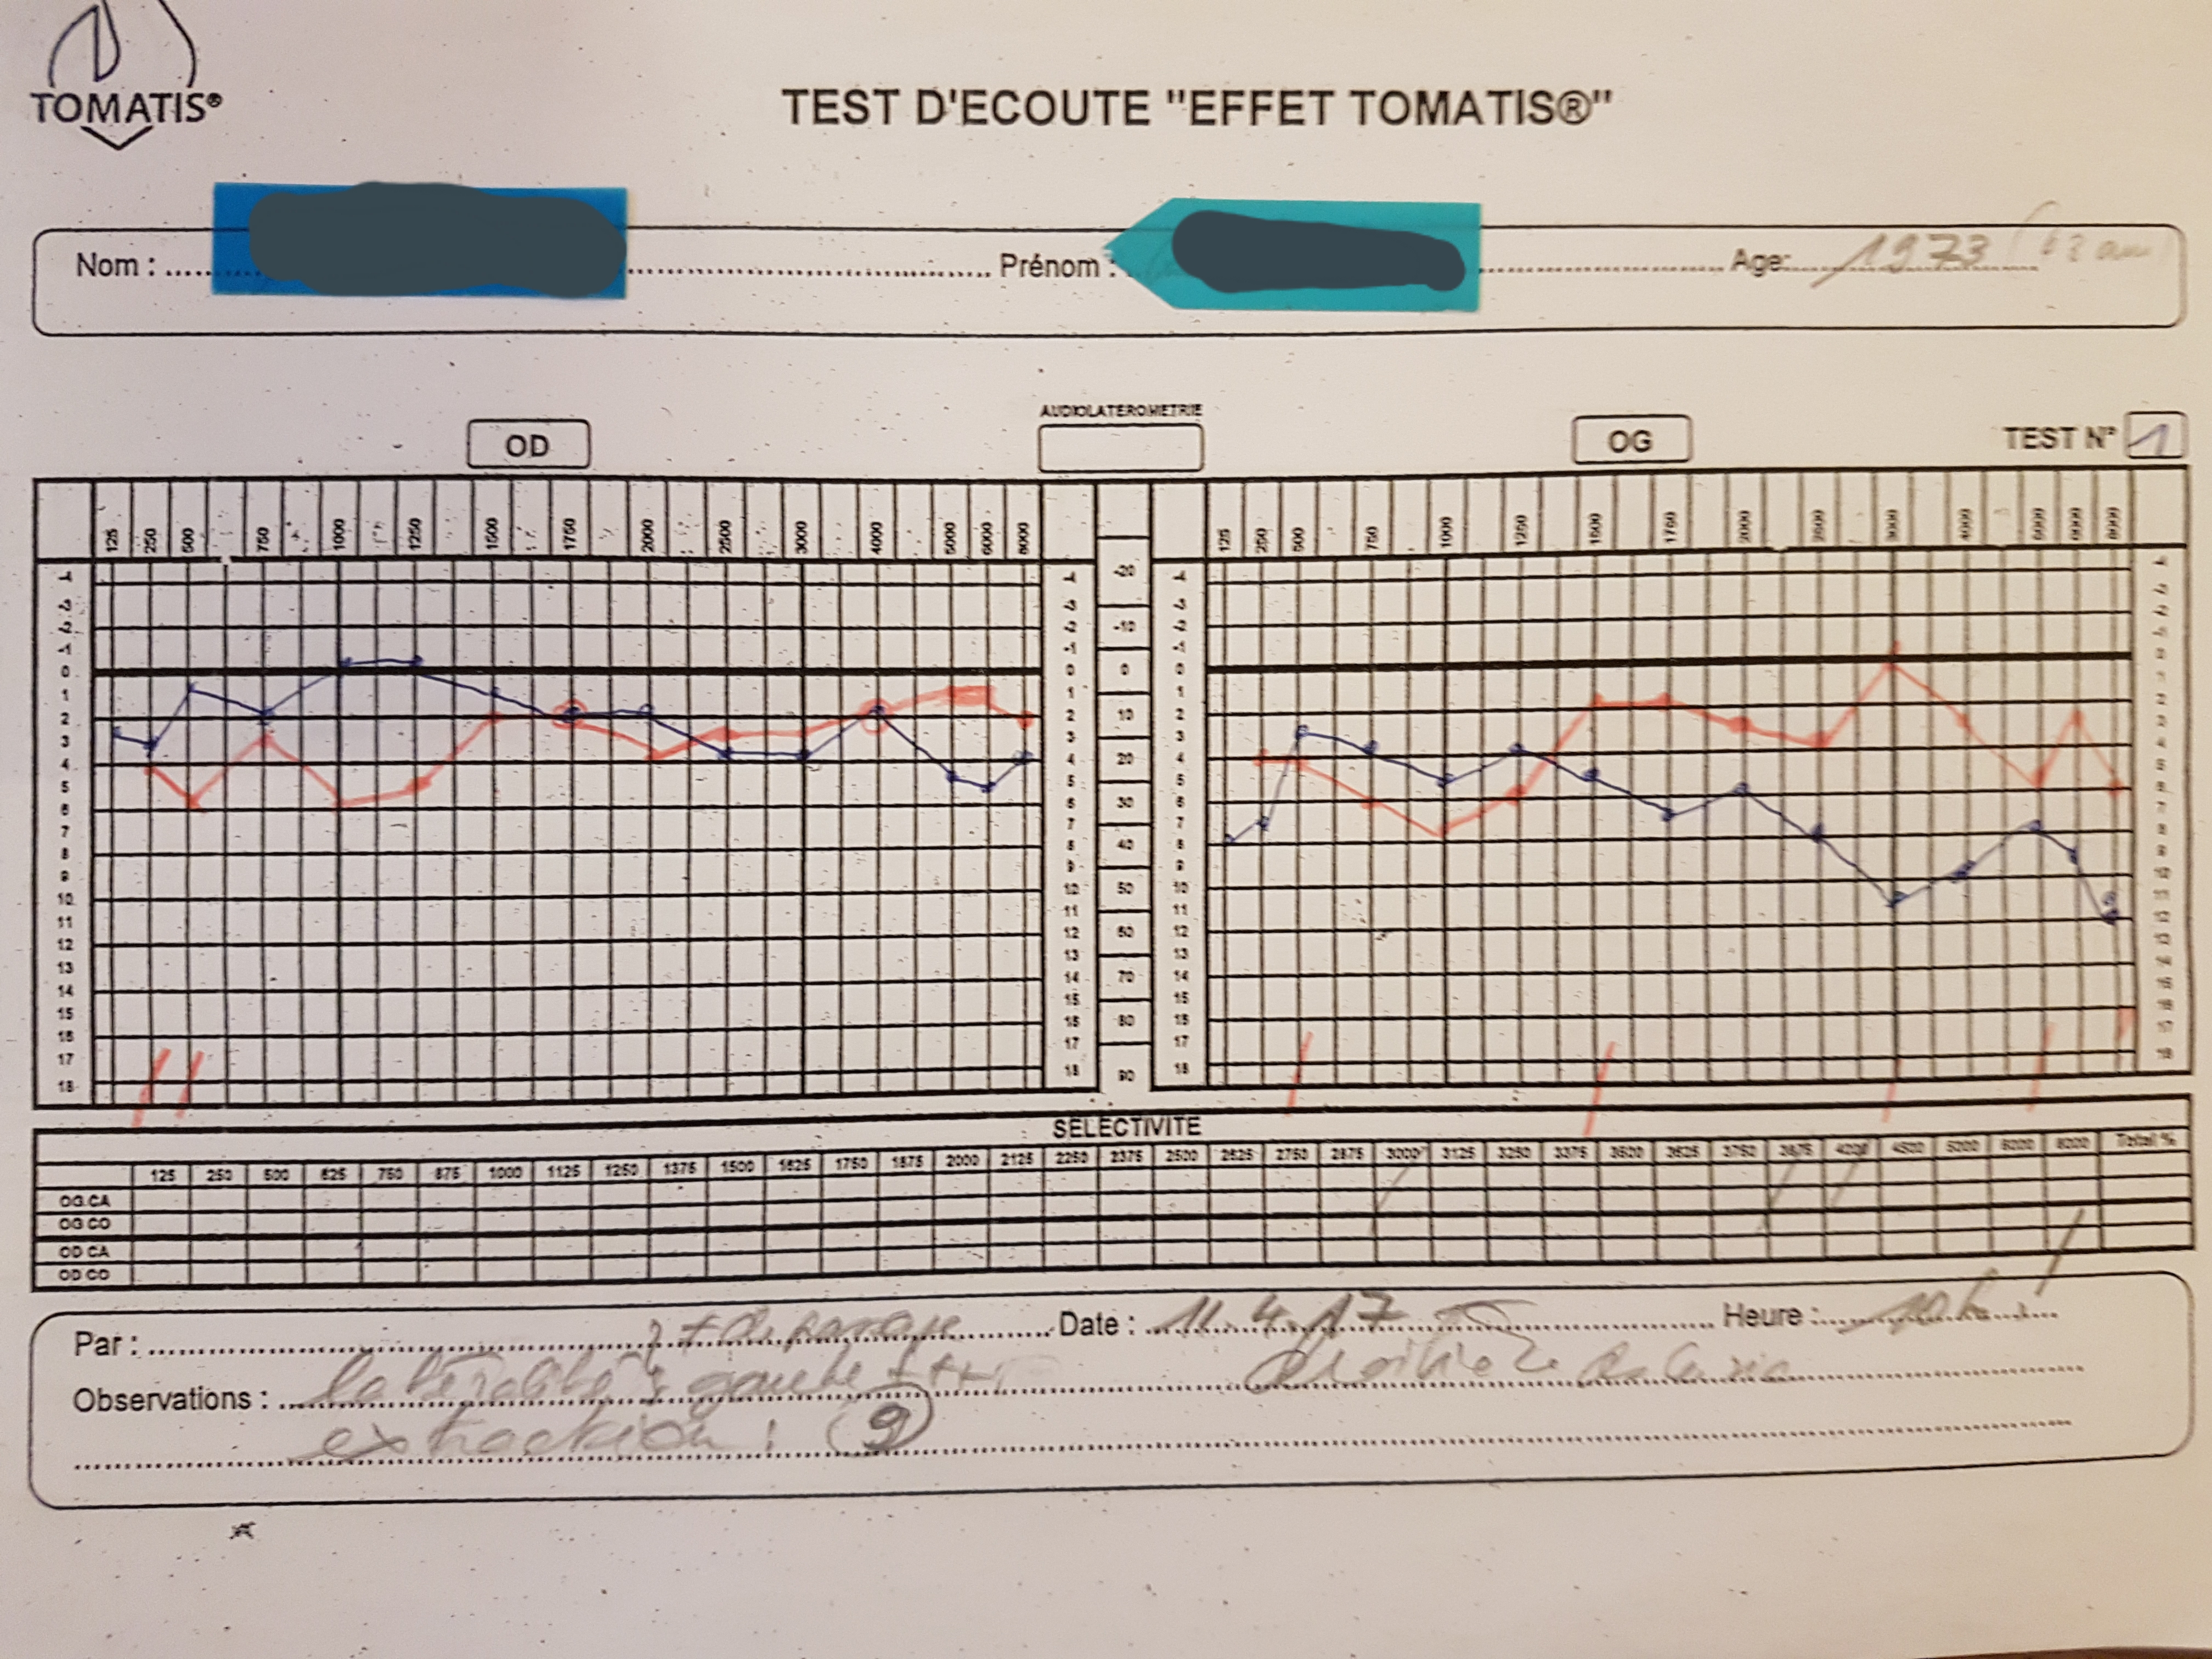
\includegraphics[width=0.7\linewidth]{images/courbesdeepressif.jpg}
	\caption{Courbes particulières d'un sujet diagnostiqué dépressif}
	\label{fig:courbes du dépressif}
      \end{figure}




      \paragraph{Descriptif selon les zones d'nterprétation:}

\begin{itemize}
  	\item Zone 1 :  Le rythme cardiaque: un stress intense va modifier le rythme
  du corps en augmentant ses fréquences. La respiration deviendra
  rapide. Il va s'en suivre une modification des perceptions
  extérieures. Une sensibilité particulièrement accrue aux bruits et
  aux sons peut en découler et être vécue comme une
  atteinte physique et psychique insupportable.
  Le changement de posture et d'attitude corporelle sont
notables (affaissement) et la perte d'énergie physique considérable (épuisement).
	\item Zone 2: La qualité de la voix: changement de la qualité du timbre de la
 voix et de l'émission verbale.	
  La voix se caractérise par son volume, son timbre, sa mélodie et son
  langage. Nous pouvons en faire le
        descriptif général, rejoignant ainsi l'idée émise lors du Congrès de la Société
américaine d'acoustique, de diagnostiquer la
        dépression par la voix:\footnote{Maryland University, 2004, 168\ieme\ Congrès de la Société
américaine d'acoustique.\autocite{le_service_metronews}. https://www.lci.fr/sante/et-si-on-diagnostiquait-la-depression-avec-u
n-test-vocal-sur-smartphone-1562728.html}.
          
 	\begin{enumerate}
 		\item le volume : basse intensité, faible dynamique
 		\item la mélodie : monotone, sans modulation
 		\item le timbre : mauvaise qualité due à une pertes des harmoniques
 		\item le langage : difficulté d'élocution, manque de fluidité
 	\end{enumerate}
        Il en découle une communication difficile avec l'entourage qui
        conduit au retrait social et à l'enfermement sur soi.
De même, un analyseur vocal peut permettre de suivre précisément l'amélioration de
l'identité vocale; sa visualisation conforte les progrès grâce aux
formants. L'enveloppe spectrale montre le timbre plus ou moins riche
dans l'empreinte vocale, renseignements précieux selon les cas.
        
	\item Zone 3: La confusion mentale, la démotivation, la perte d'énergie
psychique, la disharmonie intérieure/extérieure, le non-verbal.
\end{itemize}

 

 % \begin{figure}
%	\centering
%	\includegraphics[width=0.7\linewidth]{images/courbedepressif.jpg}
%	\caption[Exemple d'une courbe de dépressif]{Courbe
 %         représentative d'un dépressif, extrait de l'étude de Nantes,
   %      1987.}
       
%	\label{groupecontroleimage1}
%\end{figure}


	\textbf{Résonance des informations récoltées par les 3 
          zones du test d'écoute en musicothérapie et en
  psychologie :}
          
\begin{itemize}
 \item  Z.1: le physique, le corps, l'incorporation et
l'intégration du rythme,
la posture d'écoute  =  Rythme, tempo, puls 

\item  Z.2:  l'expression vocale, la communication,
l'émotionnel, la sensibilité, l'affect = Voix, timbre, mélodie 

\item Z.3: la créativité, l'interprétation, la
résonance, la musicalité, la motivation, le non-verbal (l'intraduisible en mot), l'espace = Justesse, harmonie (consonance,
dissonance), improvisation.
%\footnote{\{Hegi : L'improvisation joue un rôle centrale en musicothérapie (Hegi 1986)} 
\end{itemize}


Pour une optimalisation de l'écoute différenciée, il est souhaitable
de rejoindre dans un premier temps  le patient dans sa capacité
d'écoute de base, avec une adaptation et modulation consécutive du
volume sonore (seuils auditifs) et de l'utilisation de la voix (zone
2) en musicothérapie.
L'existence de difficultés de perception dans cette zone nous
induit à une meilleure compréhension et  élucidation de ces dernières à l'aide du
test d'écoute.

Pour élargir le concept de\textbf{ la zone 3,} comme on le
verra dans la rubrique des réflexions, nous pourrions 
également l'étendre aux notions winnicottiennes du jeu, de la capacité
créative dans un espace
intermédiaire, où l' \textit{``objet
transitionnel'' } (développé dans \textit{``Jeu et Réalité'',1953})
\autocite{winnicott} 
figure entre le ``le
dedans et le
dehors'',
l'interne et l'externe, et de là,  prolonger le questionnement du
rapport avec le concept des
courbes aérienne et osseuse.



Si on considère que ``\emph{l'alliage indissociable du corps et du psychisme, 
visible et lisible résulte de l'écoute de
sons'''}, \footnote{\emph{Extrait de l'entretien Tomatis réalisé par
  Auriol, Anvers 1973}} le concept de dépression ( R. Jouvent) \autocite{doronparot} (Cf. Annexes
A.5) inclut aussi l'idée d'une protection et une stratégie de
défense du psychisme, ayant un lien évident avec les zones du schéma d'écoute.

Même chez E.
Willems, \autocite{willems}, \footnote{  (dans sa \textit{Philosophie de la méthode} issu de sa
Pédagogie musicale) Copyright by Musique et Culture, Strasbourg} ,on relève des correspondances analogues entre les vies
corporelle (impulsions physiques)
---rythmique, affective (affection et sentiment) ---mélodique, mentale
(raisonnement et intellect)--- harmonique.


De plus, si nous nous référons à la conception indienne antique des chakras
ainsi qu'au sens de la seconde
topique de Freud (\textit{ça, moi et surmoi}), nous trouvons également des correspondances
entre les trois zones de 
fréquences et \textit{``la distribution de l'énergie pulsionnelle'}' ou entre
les 
\textit{``caractéristiques du son et l'énergie
instinctuelles''}\autocite[ch. 13]{auriol_cle_1996}.

\begin{figure}
	\centering
	\includegraphics[width=0.7\linewidth]{images/testinterpmusico}
	\caption[ L'interprétation des 3 zones et leur correspondance
        en musicothérapie]{Graphique: interprétation des 3 zones du
          test, leur correspondance en musicothérapie et selon les
          topiques de Freud.}
       
	\label{graphiquecolonnetestmusico}
      \end{figure}




%`\textit{`La mélodie est la seule forme musicale de la décharge individuelle,
%car le rythme est le moteur, pré-musical, et l'harmonie,
%supra-individuelle ``} (Mosonyi, 1835????, cité par Michel, 1965).


Ainsi, au lieu de séparer les trois grandes voies de la psychologie du
XXème siècle (psychanalyse, comportementalisme et pychologie
humaniste) comme nous le suggère T. Janssen
\autocite[197]{van_eersel_cerveau} il serait intéressant de les
considérer comme complémentaires.
%, comportant chacun un aspect qu'il
%nomme ``phénomène humain''.








      


  
 	
 	
 	
 
       
   
 





      



 











   
 

  

  
  


   
   
   
   







%\paragraph{Hypothèse}



%\paragraph{Y-a-t-il une modification de l'écoute du patient après une prise
%en charge en musicothérapie ?}
%Est-ce que le processus d'écoute en musicothérapie améliore la capacité
%d'écoute ? Devient-elle différente après une musicothérapie?

%Est-ce que les test auditifs avant et après la musicothérapie permettent
%de visualiser l'action de la musicothérapie?


%\paragraph{Est-ce que les résultats ($=$ un changement dans l'écoute) d'une prise
%en charge musicothérapeutique peuvent être lisibles et visibles dans
%un test d'écoute?}
%Est-ce possible d'évaluer un travail musicothérapeutique au moyen
%d'un test d'écoute?
%Est-ce que ces résultats sont significatifs? 

%\paragraph{Est-ce que l'écoute du patient s'est modifié ? si on a pu observer
%une modification, dans quel sens va -t-elle ?}

%Le contexte: 
%est-ce que le contexte est suffisant pour
%ressortir des résultats ?





